\documentclass[a4paper, 12pt]{article}
\usepackage[a4paper,top=1.5cm, bottom=1.5cm, left=1cm, right=1cm]{geometry}
\usepackage{cmap}					% поиск в PDF
\usepackage{mathtext} 				% русские буквы в формулах
\usepackage[T2A]{fontenc}			% кодировка
\usepackage[utf8]{inputenc}			% кодировка исходного текста
\usepackage[english,russian]{babel}	% локализация и переносы

\usepackage{amsmath}
\usepackage{indentfirst}
\usepackage{longtable}
\usepackage{graphicx}
\usepackage{array}

\usepackage{wrapfig}
\usepackage{siunitx} % Required for alignment
\usepackage{subfigure}
\usepackage{multirow}
\usepackage{rotating}
\usepackage{caption}

\graphicspath{{.}}


\title{\begin{center}Лабораторная работа №2.2.1\end{center}
Исследование взаимной диффузии газов}
\author{Рожков А. В.}
\date{\today}

\begin{document}
    \pagenumbering{gobble}
    \maketitle
    \newpage
    \pagenumbering{arabic}

    \textbf{Цель работы:} 1) регистрация зависимости концентрации гелия в воздухе от времени с помощью датчиков теплопроводности при разных начальных давлениях смеси газов; 2) определение коэффициента диффузии по результатам измерений.

    \textbf{В работе используются:} измерительная установка; форвакуумный насос; баллон с газом  (гелий); вакуумметр (класс точности 0.4, $\sigma_P = 3~торр$); источник питания; магазин сопротивлений; милливольтметр ($\sigma_U = 0.01~мВ$); компьютер с программой для проведения измерений ($\sigma_t = 1~мс$).


    \section{Теоретическая часть}
        \textit{Диффузией}  называют самопроизвольное взаимное проникновение веществ друг в друга происходящее вследствие хаотичного теплового движения молекул. При перемешивании молекул разного сорта говорят о взаимной (или концентрационной) диффузии. В системе, состоящей из двух компонентов a и b (бинарная смесь), плотности потоков частиц в результате взаимной диффузии определяются законом Фика:
        \begin{equation}
            j_a = -D \frac{\partial n_a}{\partial x}, \, j_b = -D \frac{\partial n_b}{\partial x},
        \end{equation}
        где $D$ — \textit{коэффициент взаимной диффузии компонентов}. Знак <<минус>> отражает тот факт, что диффузия идёт в направлении выравнивания концентраций. Равновесие достигается при равномерном распределении вещества по объёму.

        В данной работе исследуется взаимная диффузия гелия и воздуха. Отметим, что давление и температура в системе предполагаются неизменным: $P_0 = (n_{He}+n_{Air})kT = const$, где $n_{He}$  и $n_{Air}$ -- концентрации диффундирующих газов. Поэтому для любых изменений концентраций справедливо $\Delta n_{Air} = -\Delta n_{He}$. Следовательно, достаточно ограничиться описанием диффузии одного из компонентов, например гелия.

        Приведём теоретическую оценку для коэффициента диффузии. В работе концентрация гелия, как правило, мала ($n_{He} \ll n_{Air}$). Кроме того, атомы гелия легче молекул, составляющих воздух ($m_{He} \ll m_{N_2}, m_{O_2}$), значит их средняя тепловая скорость велика по сравнению с остальными частицами. Поэтому перемешивание газов в работе можно приближенно описывать как диффузию примеси лёгких частиц He на практически стационарном фоне воздуха. Коэффициент диффузии в таком приближении равен
        \begin{equation}
            \label{D}
            D = \frac{1}{3} \lambda \langle v \rangle,
        \end{equation}
        где $\lambda = \frac{1}{n\sigma}$ -- длина свободного пробега диффундирующих частиц; $\langle v \rangle = \sqrt{\frac{8kT}{\pi m}}$ -- их средняя тепловая скорость.

        Предполагая, что процесс диффузии будет квазиостационарным, можно показать, что разность концентраций будет убывать по экспоненциальному закону
        \begin{equation}
            \label{Delta_n}
            \Delta n = \Delta n_0 e^{-t / \tau},
        \end{equation}
        где $\tau$ -- характерное время выравнивания концентраций между сосудами, определяемое следующей формулой
        \begin{equation}
            \label{Tau}
            \tau = \frac{1}{D} \frac{V_1V_2}{V_1 + V_2} \frac{L}{S}.
        \end{equation}

    \section{Модель эксперимента}
        Для   исследования   взаимной диффузии газов и измерения коэффициента взаимной диффузии  $D$  используется  два сосуда  объёмами  $V_1$ и $V_2$ ($V_1 \approx V_2$), соединенные трубкой длины $L$ и сечения  $S$. Предполагается, что сосуды заполнены смесью двух газов при одинаковом давлении, но с различной концентрацией компонентов. Вследствие взаимной диффузии, проходящей в   соединительной трубке, концентрации компонентов в сосудах с течением времени выравниваются.

        Для измерения разности  концентраций  в установке применяются датчики теплопроводности. При этом используется тот факт, что теплопроводность смеси $\kappa$ зависит от её состава. В общем случае   зависимость  $\kappa (n)$  довольно   сложна,   однако   при   малой   разности  $\Delta n$ концентраций в сосудах можно ожидать, что разность теплопроводностей будет изменяться прямо пропорционально $\Delta n:$
        \begin{equation*}
            \Delta \kappa = \kappa (n_2) - \kappa (n_1) \approx const \cdot \Delta n.
        \end{equation*}

        Эксперименты показывают, что если доля примеси гелия составляет менее 15\%, отклонение от линейной зависимости не превышает 0.5\%, что для наших целей вполне достаточно.


        При заданной мощности нагревания приращение температуры  проволочки и, следовательно, приращение её сопротивления пропорциональны теплопроводности газа. Для измерения сопротивлений используется мостовая схема, позволяющая определять разность показаний датчиков с высокой точностью. Мост балансируется при заполнении сосудов (и датчиков) одной и той же смесью. При заполнении сосудов смесями различного состава возникает «разбаланc» моста. При незначительном различии в составах смесей показания гальванометра, подсоединённого к диагонали моста, будут пропорциональны разности концентраций примеси: $U\propto\Delta \kappa \propto \Delta n$. В процессе диффузии разность концентраций убывает по закону~(\ref{Delta_n}), и значит по тому же закону изменяются во времени показания гальванометра
        \begin{equation}
            \label{U}
            U = U_0 \, e^{-t / \tau},
        \end{equation}
        где $U_0$ -- показание в начальный момент времени. Измеряя экспериментально зависимость $U(t)$, можно получить характерное время процесса $\tau$, откуда по формуле~(\ref{Tau}) определить коэффициент диффузии $D$.


    \section{Ход работы}
    \subsection{Параметры установки}
        Номер установки - 1. Схема на рисунке \ref{ustanovka}.

        \begin{figure}[ht]
            \center{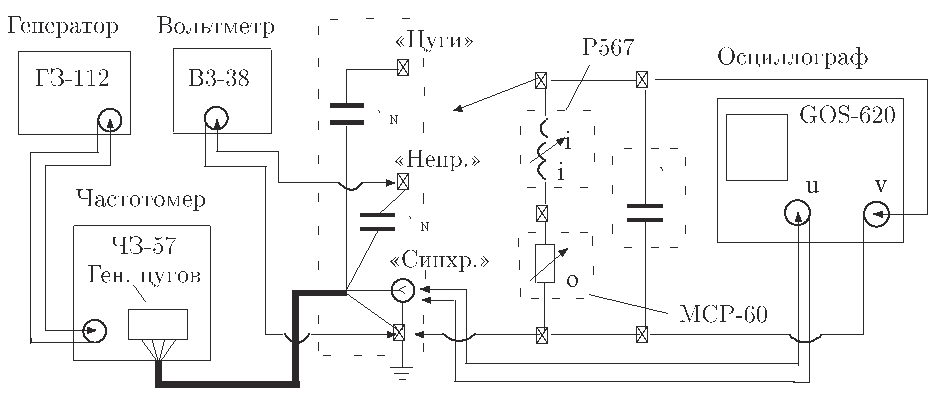
\includegraphics[scale=0.75]{pictures/ustanovka.png}}
            \caption{Схема установки 1.}
            \label{ustanovka}
        \end{figure}

        Для неё имеем:

        \begin{align*}
            V_1 = V_2 = V &= (775 \pm 10)~см^3\\
            \frac{L}{S} &= (5.3 \pm 0.1)~см^{-1}\\
            P_{атм} &= 751~торр\\
            Ц. Д. вакуумметра &= 7.43~торр
        \end{align*}

    \subsection{Подготовка установки к работе}
        а) включили питание датчиков и измерительного моста;

        б) убедились, что кран подачи гелия К7 плотно закрыт, и в установке нет
        запертых объёмов;

        в) подсоединили установку к форвакуумному насосу и откачали её до давления
        ~0.1 торр. Это достигается непрерывной работой насоса в течение
        3–5 минут (при этом показания манометра M, измеряющего разность
        давление между установкой и атмосферой, достигли максимума);

        г) после окончания откачки выключили насос.

    \subsection{Балансировка измерительного моста при рабочем давлении}

        Для начала выберем $P_{\Sigma} = 40~торр$

        а) напустили в установку воздух до давления $P_{\Sigma}$;

        б) изолировали рабочие объёмы, закрыв краны К1, К2 (К3 открыт);

        в) cбалансировали измерительный мост так, чтобы показания вольтметра флуктуировали в среднем около нулевого значения. Использовали последовательно ручки регулировки «грубо», затем «точно». После балансировки и до окончания измерений при данном $P_{\Sigma}$ положения ручек регулировки не меняли. Удалось добиться флуктуаций значений напряжения в пределах $0.01~мВ$.

    \subsection{Приготовление рабочих смесей}

        В сосуде $V_2$ должен оказаться чистый воздух, в $V_1$ смесь воздуха с гелием. Давления в сосудах должны быть одинаковы и равны рабочему $P_{\Sigma}$. Для этого выполнили следующие действия:

        а) Откачали всю установку до $\approx 0.1~торр$.

        б) Изолировали объём $V_2$, закрыв краны К2 и К3. После этого остановили откачку.

        в) Напустили в установку гелий до давления $P_{He} = 0.1P_{\Sigma}$. После этого изолировали объём $V_1$ (краном К1).

        г) Перекрыли подачу гелия (кран К7) и откачали гелий из всех патрубков. Затем остановили откачку.

        д) Присоединили объём $V_2$ к установке (кран К2) и заполнили всю установку, исключая объём $V_1$, воздухом (без гелия) до давления, избыточного по сравнению с планируемым рабочим давлением ($1.675P_{\Sigma}$).

        е) Уравняли давления в сосудах $V_1$ и $V_2$, создав поток из сосуда с воздухом в сосуд с гелием. Для этого открыли краны K1 и K2 при закрытых K3 и K4. Поскольку газ при адиабатическом расширении остывает, необходимо держать краны К1 и К2 открытыми в течение некоторого времени (30–60 с), чтобы дать давлениям выравняться при одинаковых температурах. Это время не должно быть слишком велико, чтобы диффузия гелия по патрубкам в обратном направлении не привела к искажению приготовленного состояния.

        ж) Записали точное значение установившегося рабочего давления $P_{\Sigma} = 40~торр$. Изолировали объёмы $V_1$ и $V_2$, перекрыв краны К1 и К2. Система должна быть готова к измерениям.

    \subsection{Измерение изменения теплопроводности}

        Процесс диффузии начался после открывания крана К3 . Прежде приготовили компьютерную программу по дополнительному описанию. Открыли К3 и измерили, как меняются показания вольтметра с течением времени. Измерение продолжали до тех пор, пока напряжение не упало на 50\%.

    \subsection{Измерения при различных значениях рабочего давления}

        Повторили измерения пп. 3–5 при различных значениях рабочего давления в диапазоне 40–200 торр (всего 5 значений). Графики, полученные при измерениях приведены в приложении.

    \section{Обработка результатов измерений}

    \subsection{Расчёт коэффициентов взаимной диффузии}

        Для каждого значения рабочего давления построили график зависимости $lnU(t)$.  По угловым коэффициентам и известным геометрическим параметрам установки рассчитали коэффициенты взаимной диффузии при выбранных рабочих давлениях (формулы (\ref{Tau}) и (\ref{U})). Соответствующие графики представлены в приложении. Оценили погрешности по методу наименьших квадратов. Полученные данные в таблице \ref{coeffs}.

        \begin{align*}
            \sigma_D^{приб} &= D \sqrt{\left( \frac{\sigma_{L/S}}{L/S} \right)^2 + \left( \frac{\sigma_V}{V} \right)^2 + \left( \frac{\sigma_U}{U ln \frac{U}{U_0}} \right)^2 + \left( \frac{\sigma_U}{U_0 ln \frac{U}{U_0}} \right)^2}\\
            \sigma_D &= \sqrt{\left( D \frac{\sigma_k}{k} \right)^2 + {\sigma_D^{приб}}^2}
        \end{align*}

        \begin{table}[!ht]
            \centering
            \begin{tabular}{|c|c|c|c|}
            \hline
                $P, торр$ & $\sigma_P, торр$ & $D, см^2/c$ & $\sigma_D, см^2$ \\ \hline
                40 & 3 & 11.20 & 0.28 \\ \hline
                82 & 3 & 5.54 & 0.14 \\ \hline
                119 & 3 & 3.72 & 0.10 \\ \hline
                160 & 3 & 2.83 & 0.08 \\ \hline
                201 & 3 & 2.20 & 0.05 \\ \hline
            \end{tabular}

            \caption{Результаты расчётов $D$ для каждого значения рабочего давления}
            \label{coeffs}
        \end{table}

    \subsection{Расчёт коэффициента взаимной диффузии при атмосферном давлении}

        Построили график зависимости коэффициента диффузии от обратного давления в координатах $D(1/P)$. График представлен в приложении. Экстраполируя график к атмосферному давлению, оценили соответствующий коэффициент диффузии.

        \begin{align*}
            D_{атм} &= 0.60~см^2/с\\
            \sigma_{D_{атм}} &=  \sqrt{ D_{атм}^2 \left( \left( \frac{\sigma_k}{k} \right)^2 + \left( \frac{\sigma_P}{P} \right)^2 \right) + \sigma_b^2} = 0.04~см^2/с
        \end{align*}

        Результат совпадает с табличным значением $D_{табл} = 0.62~см^2/с$ в пределах погрешности.

    \subsection{Оценка длины свободного пробега атомов гелия в воздухе и эффективного сечения столкновений атомов гелия с молекулами воздуха}

        При помощи формулы (\ref{D}) определим $\lambda_{He}$ и $\sigma_{He-возд}$ при атмосферном давлении $P_{атм} = 751~торр$ и температуре $T = 299~K$:

        \begin{align*}
            \lambda_{He} &= 142~нМ\\
            \sigma_{\lambda_{He}} &= \lambda_{He} \sqrt{\left( \frac{\sigma_D}{D} \right)^2 + \left( \frac{1}{2} \frac{\sigma_T}{T} \right)^2} = 11~нМ\\
            \sigma_{He-возд} &= 386 * 10^{-21}~м^2\\
            \sigma_{\sigma_{He-возд}} &= \sigma_{He-возд} * \sqrt{\left( \frac{\sigma_T}{T} \right)^2 + \left( \frac{\sigma_{P_{атм}}}{P_{атм}} \right)^2 + \left( \frac{\sigma_{\lambda_{He}}}{\lambda_{He}} \right)^2} = 29 * 10^{-21}~м^2
        \end{align*}

    \section{Вывод}

        Мы зарегистрировали зависимость концентрации гелия в воздухе от времени с помощью датчиков теплопроводности при разных начальных давлениях смеси газов, а также определили коэффициенты диффузии.

    \section{Приложение}

        \begin{minipage}{0.47\textwidth}
            \includegraphics[width=1\linewidth]{graphs/raw40.png}
        \end{minipage}
        \begin{minipage}{0.47\textwidth}
            \includegraphics[width=1\linewidth]{graphs/raw82.png}
        \end{minipage}

        \begin{minipage}{0.47\textwidth}
            \includegraphics[width=1\linewidth]{graphs/raw119.png}
        \end{minipage}
        \begin{minipage}{0.47\textwidth}
            \includegraphics[width=1\linewidth]{graphs/raw160.png}
        \end{minipage}

        \begin{minipage}{0.47\textwidth}
            \includegraphics[width=1\linewidth]{graphs/raw201.png}
        \end{minipage}

        \begin{figure}[ht]
            \center{\includegraphics[scale=0.6]{graphs/log.png}}
            \caption{Графики зависимости $(ln U/U_0)(t)$}
        \end{figure}

        \begin{figure}[ht]
            \center{\includegraphics[scale=0.6]{graphs/D(p^-1).png}}
            \caption{График зависимости $D(1/P)$}
        \end{figure}
\end{document}
